\documentclass{CUP-JNL-DTM}%

%%%% Packages
\usepackage{graphicx}
\usepackage{multicol,multirow}
\usepackage{amsmath,amssymb,amsfonts}
\usepackage{mathrsfs}
\usepackage{amsthm}
\usepackage{rotating}
\usepackage{appendix}
\usepackage[numbers]{natbib}
\usepackage{ifpdf}
\usepackage[T1]{fontenc}
\usepackage{newtxtext}
\usepackage{newtxmath}
\usepackage{textcomp}
\usepackage{xcolor}
\usepackage{lipsum}
\usepackage[colorlinks,allcolors=blue]{hyperref}
\usepackage{jlcode} % for rendering Julia code

%% formatting
\newtheorem{theorem}{Theorem}[section]
\newtheorem{lemma}[theorem]{Lemma}
\theoremstyle{definition}
\newtheorem{remark}[theorem]{Remark}
\newtheorem{example}[theorem]{Example}
\numberwithin{equation}{section}

% define how to display Julia
\newcommand{\Julia}{\texttt{Julia} }

% Add line numbers
% \usepackage{lineno}
% \linenumbers

%\jname{Physics/Math}
\articletype{CAPSTONE PROJECT}
%\artid{20}
%\jyear{2022}
%\jvol{}
%\jissue{}
%\raggedbottom


\begin{document}

\begin{Frontmatter}

\title[Article Title]{Using Scientific Machine Learning to solve Partial Differential Equations}

\author{Miles Cochran-Branson}\orcid{0000-0002-8514-4315}
% \author[2]{Author Name2}\orcid{0000-0001-8823-831X}
% \author[2]{Author Name3}\orcid{0000-0002-0251-345}

\authormark{M. Cochran-Branson}

\address{\orgdiv{Department of Physics and Mathematics}, \orgname{Lawrence University}, \orgaddress{\city{Appleton}, \state{WI}}}%, \postcode{54911}, \country{USA}}}

%\address[2]{\orgdiv{Division}, \orgname{Organization}, \orgaddress{\city{City}, \postcode{Pincode}, \state{State},  \country{Country}}. \email{name2@email.com}}

\abstract{Machine learning and artificial intelligence have been used with great success in data science, mathematics, and physics as well as numerous other fields to solve complex or previously impossible problems. Computationally intensive problems in physics such as data analysis using a complex model and little data, or finding numerical solutions to differential equations have traditionally been solved with classical scientific computing techniques such as Taylor-series expansions or approximations using polynomials. Recent efforts have gone into replacing these techniques with neural networks and machine learning. Neural networks have the potential to fit any complex model or differential equation solution very accurately and can solve these problems quickly. In the following paper, we describe the basic principles of the growing field of Scientific Machine Learning (SciML).
(THIS WILL LIKELY CHANGE WITH MATURITY OF THE PROJECT): We will use the techniques we describe to solve the Einstein field equations to obtain the Schwarzschild metric using the package \texttt{NeuralPDE.jl} in the \Julia programming language. This example demonstrates the power a physics-informed neural network has in solving large, highly coupled systems of partial differential equations. }

\keywords{SciML, Scientific Computing, ML/AI, PINN, PDEs}

\end{Frontmatter}

\localtableofcontents

%% ---------------------------------------------------------------
%% SECTION: INTRODUCTION
%% ---------------------------------------------------------------

\section{Introduction}

An initiative laid out by the DOE in 2019 outlines the importance and potential of the ever growing field of SciML \cite{bakerWorkshopReportBasic2019}. In this report, they indicate the computational challenges SciML could potentially solve: lack of data in analysis, and solving differential equations. In the first case, in problems where data is either expensive or impossible to collect, implementations of machine learning become impossible. This can be overcome if we can incorporate physics knowledge of the system into the neural network. Such implementations make use of \emph{Physics-Informed Neural Networks} (PINN) \cite{karniadakisPhysicsinformedMachineLearning2021}. Moreover, PINN can additionally solve differential equations by slight modification of the process used above. In fact, we can even combine these two techniques by including data into solving differential equations to better fit a model or aid in solving the equation(s). 

A robust implementation of many of these techniques has been underway in the \Julia programming languages. Packages that make use of machine learning are part of the \texttt{SciML.jl} universe which includes a basic syntax for code and basic functions in using SciML. Further information on the SciML universe can be found in last year's SciML Con \cite{SciMLCon2022}. Because of the rapidly growing nature of this field, documentation on how the techniques are used and the new tools available are not easy to access. This paper seeks to fill in some of the gaps, describing succinctly how SciML can be used to solve differential equations. In particular, we put the newly-released package \texttt{NeuralPDE.jl} to the test to solve the Einstein Field equations. 

In section two, we will outline the basics of what machine learning is. In sections three and four we will describe how to solve ODEs and PDEs with Physics-Informed Neural Networks (PINN). Finally, in section five we present a specific problem: solving Einstein's field equations to obtain the Schwarzschild Metric using the \Julia library \texttt{NeuralPDE.jl}. 

ADD HERE ONCE COMPLETED:
In the conclusions section I describe some future directions of this research and hopefully some suggestions? We shall see. Also findings?

%% ---------------------------------------------------------------
%% SECTION: MACHINE LEARNING
%% ---------------------------------------------------------------

\section{Machine Learning}

Machine learning and artificial intelligence are prominent features of our everyday life from personalized advertisements to facial recognition software. Machine learning is also a powerful analytical tool in scientific research, in particular with model development and validation. Below, I will describe how neural networks can be trained to make predictions and give some motivation for why neural networks are well suited for function approximation. 

%% SUBSECTION: NEURAL NETWORKS %%

\subsection{Neural Networks}

A neural network is simply a function. This function is composed primarily of layers of matrix multiplication, but also includes non-linear components, and optionally addition of biases \cite{strangLinearAlgebraLearning2019, bishopPatternRecognitionMachine2006}. As input, a neural network can take a scalar, vector, matrix, or sometimes tensor with a user-specified size / dimension and gives as an output a vector or scalar of weights. Thus, our network takes the form

\begin{equation}
    N : \mathbb{R}^{N} \rightarrow \mathbb{R}^{\ell}
\end{equation}
where $N$ is the user-defined input space, and $\ell$ is the number of desired output features. Networks have a fixed size defined by the number of \emph{hidden layers} and the number of \emph{nodes} each hidden layer has. 

Hidden layers are composed of nodes which cannot be directly accessed in the training process. A node within a layer describes a connection point between layers. Connections are achieved via a multiplication by a weight stored in the network. Modification of these weights changes the way in which nodes are connected to each other and thus how inputs are interpreted by the network. At each node, the weight passed to the node is modified by a non-linear function called the \emph{activation function}. This allows us to describe a complex input space more accurately \cite{dubeyActivationFunctionsDeep2022a}. Some examples of activation functions include the sigmoid defined by 

\begin{equation}
    \sigma(w) = \frac{1}{1 + e^{-w}},
\end{equation}
the hyperbolic tangent $\tanh(w)$, and LSTM defined by $f(w) = \textrm{max}\{0,x\}$ where in each case $w$ are a vector of weights of the network at a node. In examples presented later, we typically use a sigmoid activation function. 

An example of a simple neural network with one hidden layer is shown in Fig. \ref{fig:NNexample}. This network has one input dimension and, as shown in the graphic, we feed one data point $X$ with two features $x_1, x_2$ into the network. Parameters of the network are stored in the matrix $W_0$ such that when we do the multiplication $X W_0$ we get a vector of three values corresponding to the three nodes of the single hidden layer. The activation function is now applied to these values and optionally a bias vector can be added to these modified weights. We then multiply by the weights $W_1$ to get our output of a single value which is passed to one final activation function. In most cases, the activation in the final node is the identity function $f(x) = x$. Notice that we can have as many inputs, layers, nodes, and output nodes as we would like. The network described above is typically called a \emph{feed-forward} neural network as there are no cycles between nodes and no reference to nodes previously touched. There are more complex neural networks such as recurrent neural networks which have these features, however, we will not use these in our work.

\begin{figure}
\centering
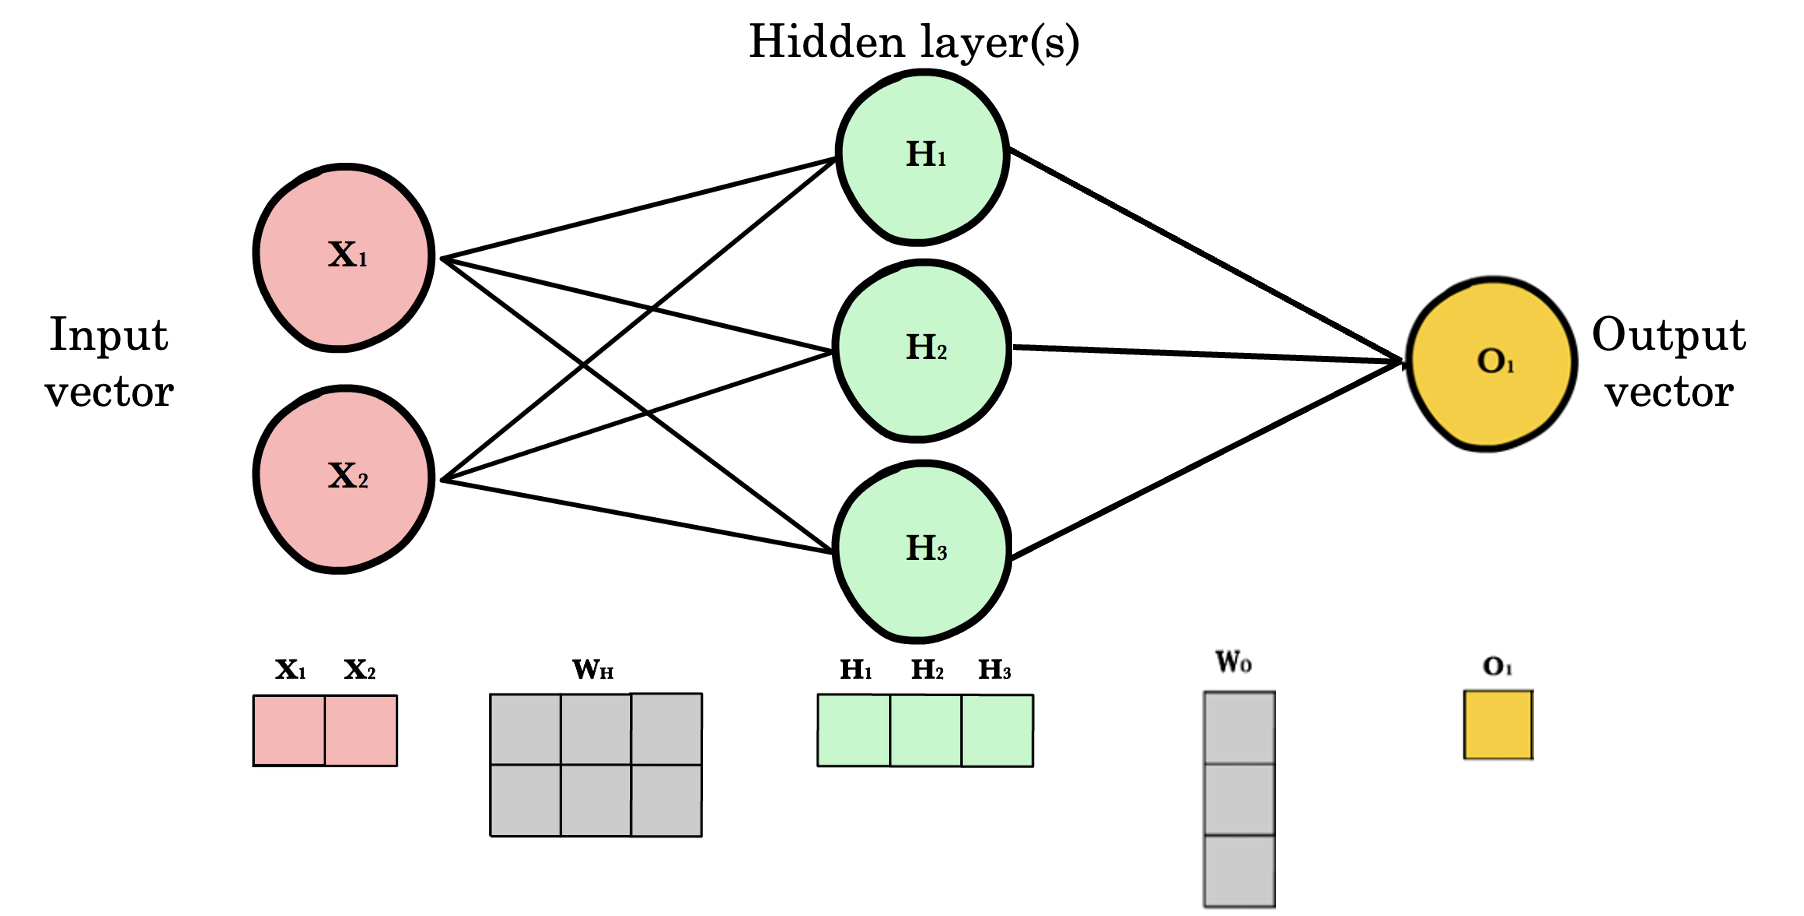
\includegraphics[width=0.7\linewidth]{figures/NN_example.png}
\caption{An example of a simple neural network with two inputs, one hidden layer with three nodes, and a single output. The network is defined by the weights connecting the layers which are represented as matrices. At each node, the weights are passed to a function called the activation function which scales the weights appropriately. In principle, the size of the network can change in every dimension. }
\label{fig:NNexample}
\end{figure}


%% SUBSECTION: TRAINING NEURAL NETWORKS %% 

\subsection{Training Neural Networks}

Now that we have built some neural network, we would like to have it make some useful predictions! This involves picking a set of special weights through a process called training. 

In order to train a neural network, we need a way in which to evaluate how well the network is doing. This is achieved with a \emph{loss function}. The loss function takes an input of all of the parameters of the network that can change, $X$, and outputs a single number, thus, our loss function is of the form

\begin{equation}
    L : \mathbb{R}^{\textrm{size}(X)} \rightarrow \mathbb{R}. 
\end{equation}
Such a function is defined such that the smaller the output value, the better the network performs. Thus, training a neural network becomes an optimization problem where we want to minimize the function $L(X)$. Typically, the space $X$ is composed of the weights and biases of the network leaving the structure of the network intact. 

For a very basic idea of how this works, imagine the space defined by $L$ as a surface with some collection of minima. We want to find a minimum, so we need to travel in the direction of a minimum. In most cases, it is not necessary to find the global minimum and may even be computationally disadvantageous as finding global minimum can lead to over-fitting \cite{choromanskaLossSurfacesMultilayer2015}. Intuitively, we can take the gradient and then travel in the direction of the negative gradient to go ``downhill". 

More specifically, we travel in the $-\nabla L(X)$ direction taking discrete steps of size $\Delta x$. After each step we update the network parameters, re-evaluate the loss, compute $-\nabla L(X)$ and repeat. We continue in this way for as many steps as the user desires. This process is called gradient descent and the process of finding the desired weights is called backpropogation \cite{chauvinBackpropagationTheoryArchitectures1995}. 

Because in some cases, learning can get stuck in a saddle point or small local minimum, we often use stochastic methods which allow us to get out of such cases and continue learning to a minimum. This process is called stochastic gradient descent. In the following examples, we will use the ADAM optimizer which uses stochastic methods to find a minimum \cite{kingmaAdamMethodStochastic2017}. 

%% SUBSECTION: THE UAT %%

\subsection{The Universal Approximation Theorem}

One natural question in using neural networks to solve differential equations, is why this method works or why even it has a chance of working. The answer comes down to a famous theorem in machine learning: the Universal Approximation Theorem (UAT):

\begin{theorem}

Let $x \in \Omega$, let $u(x)$ be a regular function, and $N(x,w)$ be a neural network with weights $w$. Then, we can find some arbitrarily small $\epsilon \in \Omega$ such that 

\begin{equation}
	||N(x,w) - u(x)|| < \epsilon. 
\end{equation}

\end{theorem}

\noindent Proofs of this theorem are beyond the scope of this report, but are readily availible for several different contexts including for classical feed-forward networks \cite{hornikMultilayerFeedforwardNetworks1989, hornikApproximationCapabilitiesMultilayer1991}, finding probability distributions \cite{luUniversalApproximationTheorem2020}, and complex-valued neural networks \cite{voigtlaenderUniversalApproximationTheorem2020}. 

There is, however, one big caveat to this theorem: nothing about the problem tells us how big our network should be in order to fulfill the theorem. In some cases, the size of the network may be computationally infeasible to model. Nonetheless, it is this theorem which allows us to be able to have some hope that differential equations can be arbitrarily approximated by neural networks. 

In the rest of the paper, we describe the technicalities for solving differential equations with neural networks, starting with ODEs and moving on to solving PDEs. 

%% ---------------------------------------------------------------
%% SECTION: SOLVING ODES WITH PINN
%% ---------------------------------------------------------------

\section{Solving ODEs with Physics-Informed Neural Networks}

As an illustration of the application of PINN, consider an ordinary differential equation of the form 

\begin{equation}
	u' = f(u,t). 
\end{equation}
The UAT tells us that we should be able to achieve $N(w,t) = u(t)$ where $N(w,t)$ is a neural network with weights $w$. Consequently, our neural network must satisfy $N'(w,t) \approx f(N(w,t), t)$. To solve, we discretize the space $\Omega$ where $t \in \Omega$. Subsequently, we define the loss function by 

\begin{equation}
	L(w) = \sum_i \left( \frac{dN(w, t_i)}{dt} - f(N(w,t_i), t_i)\right)^2. 
\end{equation}
In order to find a unique solution, we apply the initial condition $u(0) = u_0$. We can simply add this to our loss function as 

\begin{equation}
	L(p) = (N(w,0) - u_0)^2 + \sum_i \left( \frac{dN(w,t_i)}{dt} - f(N(w,t_i), t_i),\right)^2
\end{equation}
or we can parametrize the function to learn on, encoding the initial condition in our neural network solution by defining the function 

\begin{equation}
	g(w,t) = u_0 - tN(w,t).
\end{equation}
This ensures that the initial condition is satisfied and allows us to write down a simpler version of the loss function:

\begin{equation}
	L(w) = \sum_i \left(\frac{dg(w,t_i)}{dt} - f(g(w,t_i), t_i)\right)^2. 
\end{equation}

Now that we have defined our problem, we can use standard techniques to solve simple ODEs. For more information and further examples see \cite{rackauckasSciMLSciMLBookParallel}. 

\subsection{Example ODE problem solved with PINN}

\begin{example}
	
Consider the equation

\begin{equation}
	u' = e^t \cos t
\end{equation}
with the initial condition $u(0) = 0.1$. Notice that we can find the solution to this equation via integration, i.e., the solution is given by

\begin{equation}
	u(t) = \int e^t \cos t \, dt. 
\end{equation}
Applying integration by parts twice, we find the solution

\begin{equation}
	u(t) = \frac{1}{2}e^t(\sin t + \cos t) + C
\end{equation}
where $C = -0.4$ via use of the initial condition. 

Let's now solve using the techniques defined above using \Julia and the machine learning package \texttt{Flux.jl}. We begin by defining a neural network with two hidden layers one of 64 nodes the other with 32 nodes using the $\tanh$ activation function and a linear output: 

\begin{jllisting}
using Flux
NNODE = Chain(x -> [x], # Take in a scalar and transform it into an array
           Dense(1,64, tanh),
           Dense(64, 32, tanh),
           Dense(32,1),
           first) # Take first value, i.e. return a scalar
\end{jllisting}
We then parametrize the solution and define the loss function in which the differential is computed via discretization:

\begin{jllisting}
g(t) = t*NNODE(t) + 0.1

using Statistics
ϵ = sqrt(eps(Float32))
loss() = mean(abs2(((g(t+ϵ)-g(t))/ϵ) - (exp(t) * cos(t))) for t in 0:1f-2:5f0)
\end{jllisting}
Notice that we use machine $\epsilon$ here to discretize our integral as this is the smallest possible meaningful discretization. We will use gradient descent to solve with a learning rate of $10^{-4}$ over $10^4$ epochs. Because there is no data we are providing to train on, we feed the network empty data. Instead, all of the learning information comes from the loss function defined above. This is accomplished with the following code:

\begin{jllisting}
epochs = 10_000
learning_rate = 1e-4

opt = Flux.Descent(learning_rate) # use gradient Descent
data = Iterators.repeated((), epochs) # no data here : repeat empty data
iter = 0
loss_history = []
cb = function () #callback function to observe training
  global iter += 1
  push!(loss_history, loss())
  if iter % 500 == 0
    display(loss())
  end
end
display(loss())
Flux.train!(loss, Flux.params(NNODE), data, opt; cb=cb)
\end{jllisting}
We can then see how our network does in comparison to the true solution as shown in the below plot:

\begin{center}
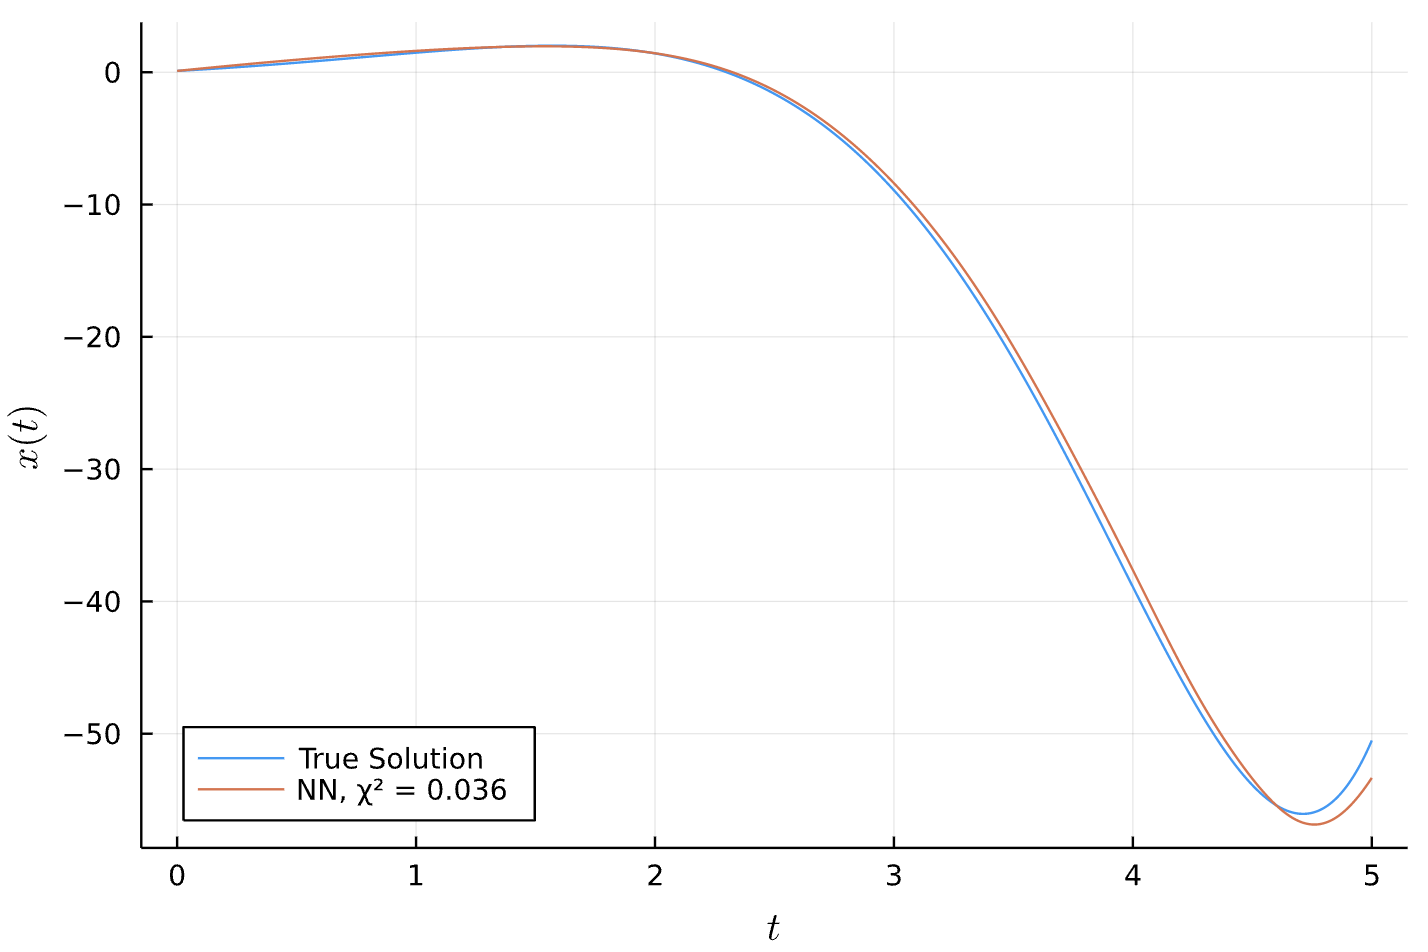
\includegraphics[width=0.45\linewidth]{figures/ODE_example.png}
\end{center}
and we see that our network does pretty well! We could, of course, improve performance by training longer or playing with the size of the network or learning rate, however the above still remains a good example of how to utilize neural networks to solve ODEs. 
	
\end{example}

%% ---------------------------------------------------------------
%% SOLVING PDES WITH PINN
%% ---------------------------------------------------------------

\section{Solving PDEs with Physics-Informed Neural Networks}

We now turn out attention to solving partial different equations using techniques from scientific machine learning. We will use the package \texttt{NeuralPDE.jl} \cite{zubovNeuralPDEAutomatingPhysicsInformed2021} to solve some examples. 

Consider a partial differential equation given by 

\begin{equation}
	f(u(x); \lambda) = 0
\end{equation}
where $x \in \Omega$ are the independent variables in the space $\Omega$, $u(x)$ is the solution, $f$ is some non-linear function acting on $u$, and $\lambda$ are the parameters of the equation. To solve with a neural network $N(x, w)$ where $N$ is a neural network with weights $w$, we want to fulfill 

\begin{equation}
	f(N(x, w); \lambda) \approx 0.
	\label{eqn:NNapprox}
\end{equation}
The universal approximation theorem tells us that this should be possible. The error of the above equation is then given by 

\begin{equation}
	L(w) = \int_{\Omega} ||f(N(x,w); \lambda)||\,dx. 
	\label{eqn:NNloss}
\end{equation}
We have suggestively named the error $L$ as we can use this function as a loss function in training our neural network $N$ by minimizing $L$. Our computational problem then reduces to the problem of evaluating the integral in Eqn. \ref{eqn:NNloss}. Notice that in practical problems, we apply boundary conditions $b_i$ on $\partial \Omega \in \Omega$. In order to use these in our neural network, we add in these conditions to our loss function giving us 

\begin{equation}
	L(w) = \sum_i\int_{\Omega\setminus\partial\Omega} ||f_i(N(x,w); \lambda)||\,dx + \sum_i\int_{\partial\Omega} ||b_i(N(x,w); \lambda)||\,dx.
	\label{eqn:complete_loss} 
\end{equation}
where we have generalized the problem to a system of coupled differential equations $f_i$. 

There are several different methods for evaluating the above integral namely: grid approximation techniques, stochastic grid approximation techniques, and machine learning (quadrature) techniques. A simple grid approximation takes the space $\Omega$ and divides it into units of volume $\Delta V$ with a specific length. The PDE is evaluated at each of this points and scaled by the volume, thus our integral is computed via 

\begin{equation}
	\int_{\Omega} ||f(N(x,w); \lambda)||\,dx = \sum_i \Delta V ||f(x_i)||.
\end{equation}
This method has two main disadvantages: 1) as the dimension of the problem increases, the number of points we sample increases exponentially in order to maintain the same granularity and 2) no evaluation of the integral is done between grid points, thus information can be quickly lost. To solve the second problem, we can use stochastic methods of sampling---i.e., use Monte Carlo techniques to evaluate the integral. This can be described by 

\begin{equation}
	\int_{\Omega} ||f(N(x,w); \lambda)||\,dx = \alpha \sum_i ||f(x_i)||.
\end{equation}
for some scaler $\alpha$. As we simply want to minimize this integral, there is no need to specify $\alpha$. This problem still suffers from dimensionality exponentially increasing. Thus, we turn to a third method: quadrature training with a neural network. Several processes for specifying quadrature are described in \cite{riveraQuadratureRulesSolving2022}. These are typically of the form 

\begin{equation}
	\int_{\Omega} ||f(N(x,w); \lambda)||\,dx = \sum_i \alpha_i ||f(x_i)||\,dx.
\end{equation}
In the implementation via \texttt{NeuralPDE.jl}, this is accomplised using the \texttt{Integrals.jl} package which calls the \Julia differential equation solver \cite{rackauckasDifferentialEquationsJlPerformant2017} to find the correct sampling points $x_i$ and weights $\alpha_i$ in an implementation of Gaussian quadrature rules. 

\subsection{Example using \texttt{NeuralPDE.jl}}

We show how \texttt{NeuralPDE.jl} can be used to solve a simple example and describe the important components of the code. 

\begin{example}

Consider the system of PDEs given by 

\begin{equation}
    \begin{split}
        \partial_t u_1 & = \partial_x^2 u_1 - u_2 \partial_x u_1 + u_1^2 - 2\int_0^1 u_1^2 \,dx \\
        0 & = \partial_x u_2 - u_1
    \end{split}
\end{equation}
for $0 < x < 1$ and $t > 0$. This system arises as a simplification of the Navier-Stokes equations in an infinitely-long channel \cite{buddBlowupSystemPartial1994}. We employ the following initial condition

\begin{equation}
    u_1(0,x) = \cos \pi x
\end{equation}
and the boundary conditions

\begin{equation}
    \partial_x u_1(t,0) = \partial_x u_1(t,1) = u_2(t,0) = u_2(t,1) = 0. 
\end{equation}
This system is solved analytically in the paper \cite{benhammoudaAnalyticalSolutionsSystems2014} where they find the exact solution

\begin{equation}
    \begin{split}
        u_1(t,x) & = e^{-\pi^2t}\cos \pi x \\
        u_2(t,x) & = \frac{1}{\pi}e^{-\pi^2t} \sin \pi x. 
    \end{split}
\end{equation}

Let's now solve this problem using \texttt{NeuralPDE.jl}. We begin by importing the required packages from \Julia, defining the variables and parameters of the system, and defining the equation, boundary conditions, and domains over which we want to solve. 

\begin{jllisting}
using NeuralPDE, ModelingToolkit, Lux, Domainsets
using Optimization, OptimizationOptimisers
import ModelingToolkit: Interval

@parameters t x
@variables u1(..) u2(..)

Dx = Differential(x)
Dxx = Differential(x)^2
Dt = Differential(t)
Ix = Integral(x in DomainSets.ClosedInterval(0, 1))

eqns = [Dt(u1(t,x)) ~ Dxx(u1(t,x)) - u2(t,x)*Dx(u1(t,x)) + 
                                        (u1(t,x))^2 - 2*Ix((u1(t,x))^2),
        0 ~ Dx(u2(t,x)) - u1(t,x)]

bcs = [u1(0,x) ~ cos(π*x),
        Dx(u1(t,0)) ~ 0,
        Dx(u1(t,1)) ~ 0,
        u2(t,0) ~ 0,
        u2(t,1) ~ 0
]

domains = [x ∈ Interval(0.0, 1.0),
            t ∈ Interval(0.0, 1.0)]

@named pde_sys = PDESystem(eqns, bcs, domains, [t,x], [u1(t,x), u2(t,x)])
\end{jllisting}
Notice that with the aid of the package \texttt{ModelingToolkit.jl}, we can symbolically represent the set-up of our problem. This is a feature of the SciML ecosystem of \Julia. 

We then create a neural network using \texttt{Lux.jl} and pick a discretization to use. In this example we use the sigmoid as our activation function and build a network with one hidden layer of fifteen nodes. The input layer of our network must be the length of the number of parameters defined in our problem. Additionally, we use a different neural network for each solution $u_1$ and $u_2$ of our system, thus we define two neural networks with the set-up described above. The discretization we choose is the quadrature training method described above. 

\begin{jllisting}
dim = length(domains) # number of dimensions
n = 15
chains = [Lux.Chain(
            Dense(dim, n, Lux.σ), 
            Dense(n, n, Lux.σ), 
            Dense(n, 1)) for _ in 1:2]

strategy = QuadratureTraining()
discretization = PhysicsInformedNN(chains, strategy)
@time prob = discretize(pde_sys, discretization)
\end{jllisting}

We finally define a function to record the loss of our training and train the network

\begin{jllisting}
i = 0
loss_history = []

callback = function (p,l)
    global i += 1
    if i % 100 == 0
        println("Current loss is: $l")
    end
    append!(loss_history, l)
    return false
end

res = @time Optimization.solve(prob, ADAM(0.1); 
                                callback = callback, maxiters=500)
prob = remake(prob, u0=res.minimizer)
res = @time Optimization.solve(prob, ADAM(0.01); 
                                callback = callback, maxiters=2000)
prob = remake(prob, u0=res.minimizer)
res = @time Optimization.solve(prob, ADAM(0.0001); 
                                callback = callback, maxiters=2000)
\end{jllisting}
For optimization we use the ADAM optimizer and vary the learning rate starting with a rate of 0.1 over 500 epochs, then 0.01 over 2000 epochs, then finally $10^{-4}$ over a final 2000 epochs. The loss over these epochs and learning rates is shown below

\begin{center}
    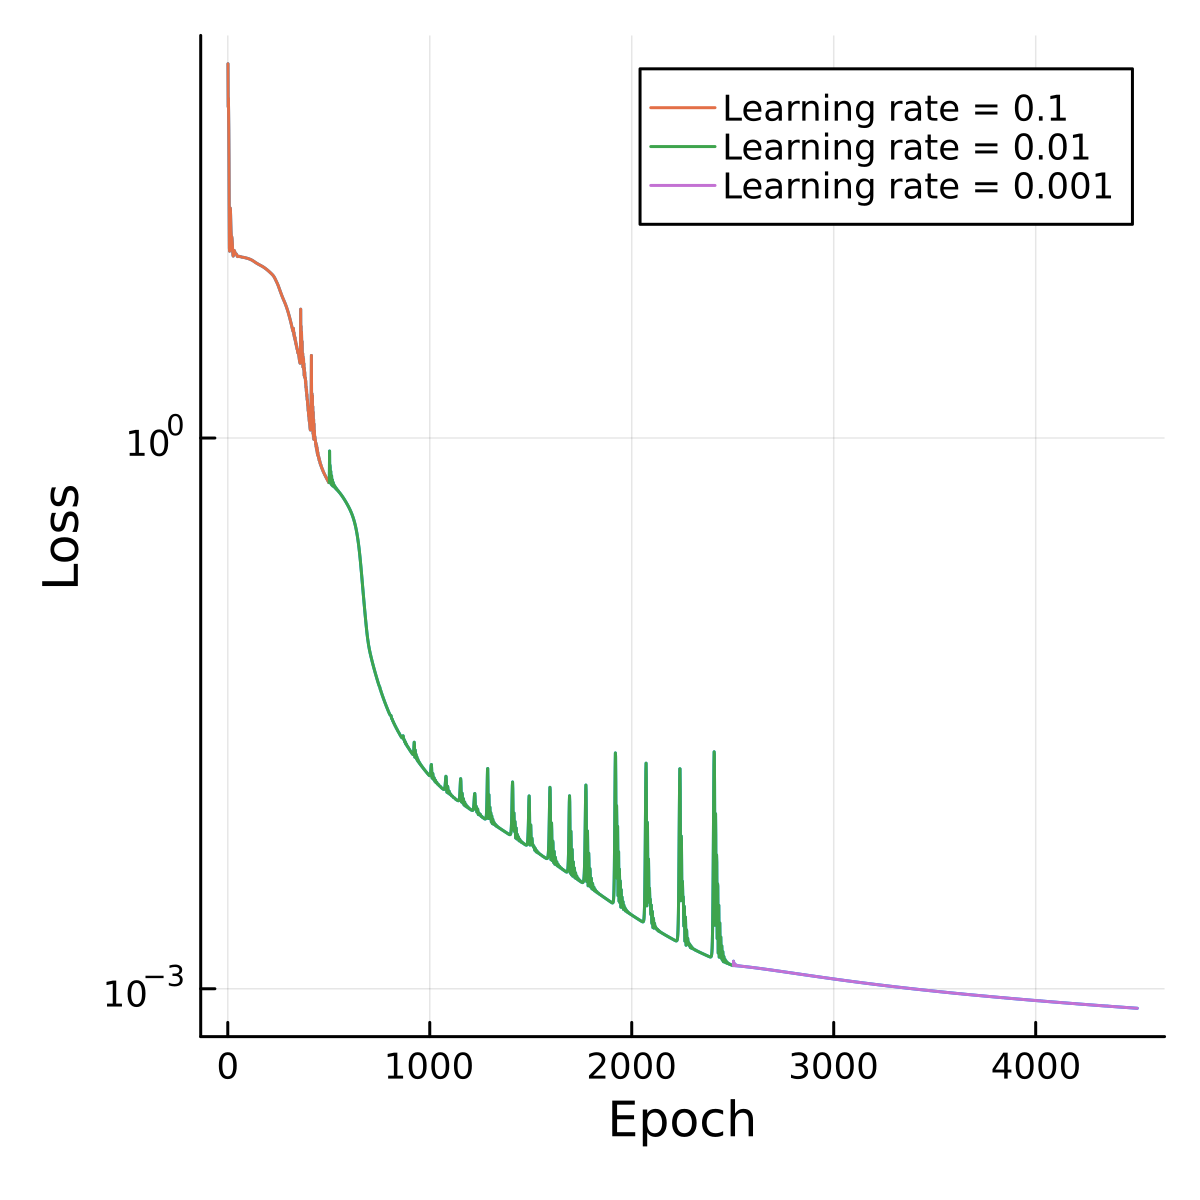
\includegraphics[width=0.3\linewidth]{figures/integral_PDE_plots/loss.png}
\end{center}

We can then plot the result of this training as shown below:

\begin{center}
    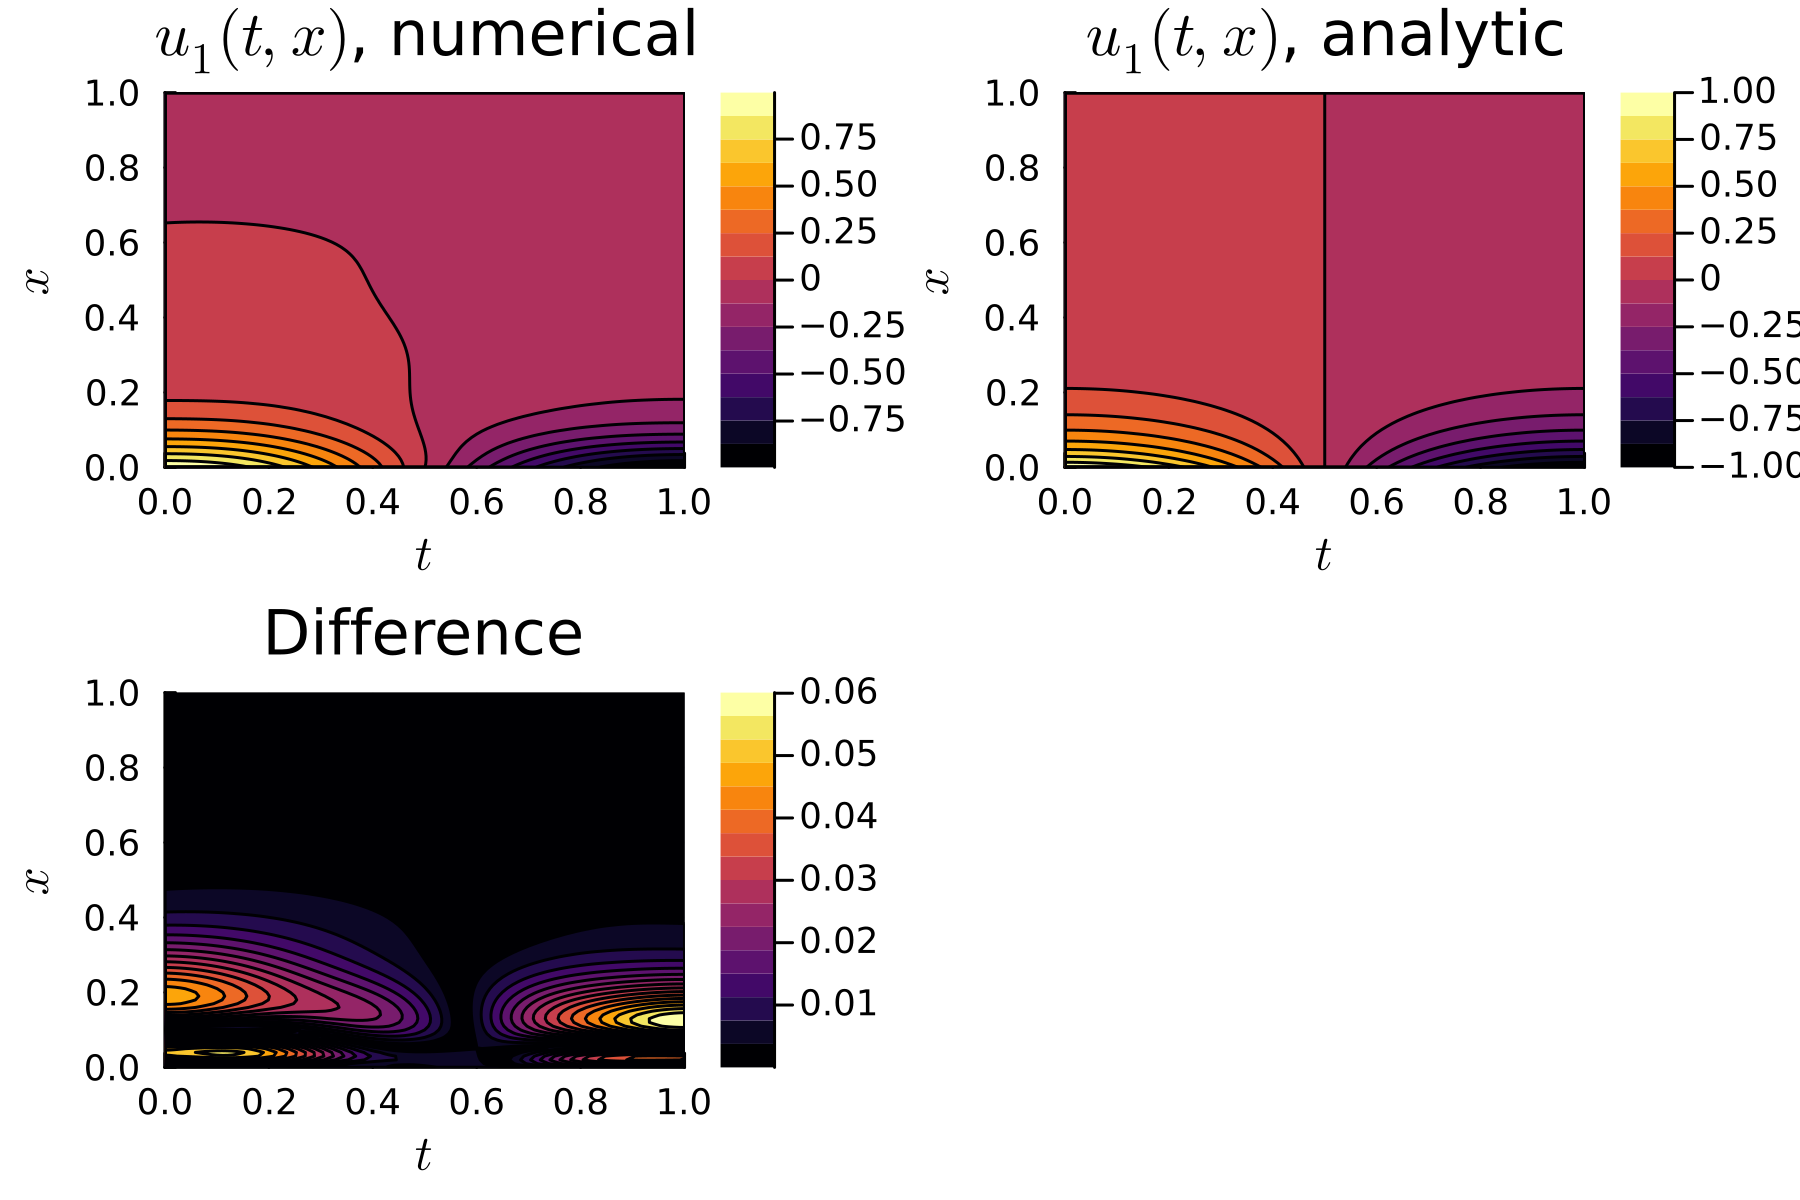
\includegraphics[width=0.48\linewidth]{figures/integral_PDE_plots/plot_u1.png}
    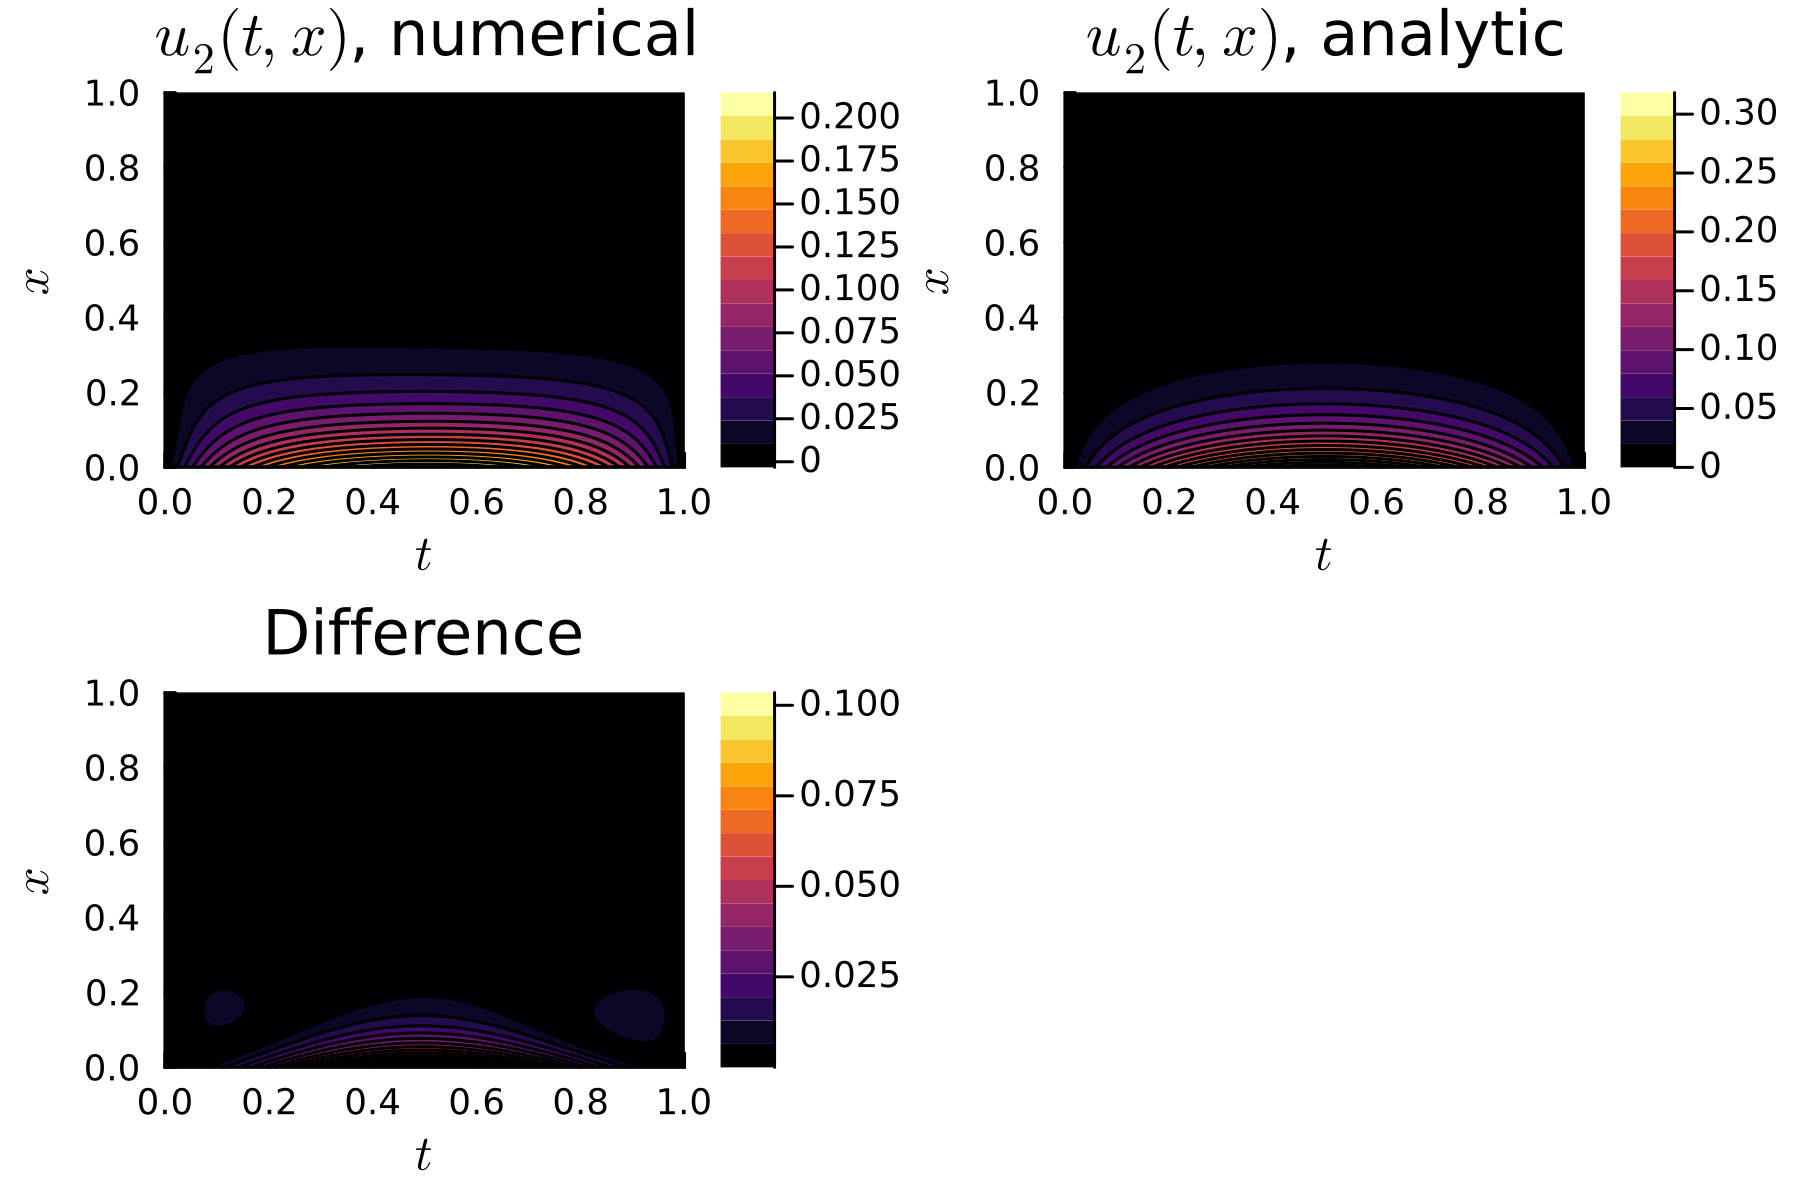
\includegraphics[width=0.48\linewidth]{figures/integral_PDE_plots/plot_u2.png}
\end{center}
and we see that our numerical solution very closely matches the analytical solution. 

For more information, see the data availability statement. 

\end{example}

%% ---------------------------------------------------------------
%% SECTION: SOLVING EFE
%% ---------------------------------------------------------------

\section{Solving Einstein's Field Equations to obtain the Schwarzschild Metric using \texttt{NeuralPDE.jl}}

\subsection{Physics Background and Problem Set-up}

We find a solution to Einstein's field equations under a few assumptions to yield the Schwarzschild Metric as first described by Schwarzschild in 1916 \cite{schwarzschildGravitationalFieldMass1999}. 

Einsteins field equations are given by 

\begin{equation}
    R_{\mu\nu} - \frac{1}{2}R g_{\mu\nu} + \Lambda g_{\mu\nu} = \frac{8 \pi G}{c^4}T_{\mu\nu}
    \label{eqn:EFE}
\end{equation}. 

Under our assumptions (Define) this reduces to 

\begin{equation}
    R_{\mu\nu} = 0. 
\end{equation}

We define connecting coefficients as 

\begin{equation}
    \Gamma^{\alpha}_{\mu\nu} = -\frac{1}{2}\sum_{\beta}g^{\alpha\beta}\left(\frac{\partial g_{\mu\beta}}{\partial x_{\nu}} + \frac{\partial g_{\nu\beta}}{\partial x_{\mu}} - \frac{\partial g_{\mu\nu}}{\partial x_{\beta}}\right)
    \label{eqn:ccs}
\end{equation}
The solutions outlined in Swarzschild's paper yields the following differential equations to solve

\begin{equation}
    \sum_{\alpha} \frac{\partial \Gamma^{\alpha}_{\mu\nu}}{\partial x_{\alpha}} + \sum_{\alpha\beta} \Gamma^{\alpha}_{\mu\beta} \Gamma^{\beta}_{\mu\alpha} = 0
\end{equation}
where we also require 

\begin{equation}
    |g_{\mu\nu}| = -1. 
\end{equation}

A full solution to this problem yielding the analytic solution in spherical coordinates

\begin{equation}
    g_{\mu\nu} = \begin{pmatrix}
        1 - \frac{r_s}{r} & 0 & 0 & 0 \\
        0 & -(1 - \frac{r_s}{r})^{-1} & 0 & 0 \\
        0 & 0 & r^2 & 0 \\
        0 & 0 & 0 & r^2\sin^2\theta
    \end{pmatrix},
\end{equation}
where 

\begin{equation}
    r_s = \frac{2GM}{c^2},
\end{equation}
is given in \cite{eigenchrisRelativity108aSchwarzschild}. 

\subsection{Technical Implementation}

\subsection{Results and Discussion}

%% ---------------------------------------------------------------
%% SECTION: CONCLUSION
%% ---------------------------------------------------------------

\section{Conclusion}

%% ---------------------------------------------------------------
%% BACKBATTER, MISC. 
%% ---------------------------------------------------------------

\begin{Backmatter}

\paragraph{Acknowledgments}

I am very grateful for the mentorship of Alex Heaton and Megan Pickett in working on this project. Additionally, none of this would have been possible without the education I have received at Lawrence University. I would like to thank the Physics and Mathematics department for their support and all of the opportunities I have had through both departments. 

\paragraph{Data Availability Statement} All code presented above can be found here in GitHub at the following link \texttt{https://github.com/lvb5/solve\_PDEs\_with\_PINN}. 

\bibliography{references}
\bibliographystyle{ieeetr}

\end{Backmatter}

\end{document}

%% EXTRA EXAMPLE

% \begin{example}

% Consider the PDAE given by 

% \begin{equation}
%     \begin{split}
%         \partial_t^2 u_1 & = \partial_x^2 u_1 + u_3 \sin \pi x \\
%         \partial_t^2 & = \partial_x^2 + u_3 \cos \pi x \\
%         0 & = u_1 \sin \pi x + u_2 \cos \pi x - e^{-t}
%     \end{split}
% \end{equation}
% on the intervals $0 < x < 1$, $t > 0$. We require the initial conditions

% \begin{equation}
%     \begin{split}
%         u_1(0,x) & = \sin \pi x \\
%         \partial_t u_1(0,x) & = -\sin \pi x \\
%         u_2(0,x) & = -\sin \pi x \\
%         \partial_t u_2(0,x) & = -\cos \pi x
%     \end{split}
% \end{equation}
% and the boundary conditions

% \begin{equation}
%     \begin{split}
%         u_1(t,0) & = u_1(t,1) = 0 \\
%         u_2(t,0) & = -u_2(t,1) = e^{-t}. 
%     \end{split}
% \end{equation}
% The exact solution to this system is given by 

% \begin{equation}
%     \begin{split}
%         u_1(t,x) & = e^{-t}\sin \pi x \\
%         u_2(t,x) & = e^{-t}\cos \pi x \\
%         u_3(t,x) & = (1+\pi^2)e^{-t}
%     \end{split}
% \end{equation}
% for $0 \le x \le 1$, $t \ge 0$. 

% \end{example}
